% !TEX root = ../Article.tex
\chapter{Background}
In this chapter we will provide the background information necessary to understand how smart cards function and how they increase security on mobile devices. In particular, we will cover smart card technology, relevant mobile device technology (in our case Android OS), basic concepts of cryptography and typical threats in the context of mobile devices.
%The topics covered in this section are smart cards, mobile device operating systems, cryptography and threats in context of mobile devices.

\section{Smart card}
\label{sec:smartcard}
The term smart card refers to a card with an integrated circuit. In essence a smart card is a miniature computer with limited computing power. In practice, it is a miniature computer with limited computing power, which can process information in a secure isolated environment and exchange data with the device that usually also provides it with the necessary power to operate.

\subsection{Smart card architecture}
The micro processor is able to perform tasks that involve processing input, give ouput and storing small amounts of data. Smart cards vary in sizes defined by the standards ISO/IEC 7810 \cite{iso7810} and ISO/IEC 7816 \cite{iso7816}. The most common card dimensions are approximately 85x54 mm \cite[~Ch. 3.1]{smartcardHandbook}. The processing power of smart cards are between 25-32 MHz and sport anywhere from 8Kbit to 128Kbit memory (EEPROM) \cite{cardProcessing}.

The micro processor can be powered and communicate in two ways. Contact smart cards have integrated contact pads. When the smart card is inserted into a card reader the contact pads of the card reader provides power to the micro processor via the contact pads of the smart card. The contact pads also functions as a medium for transferring data. Contactless smart cards uses radio-frequency induction to power the micro processor and to transmit data between an antenna and the card. Most modern smart cards supports both technologies (hybrid cards). Figure \ref{fig:nfccard} shows a contact smart card and reader.

An everyday example of a smart card is the modern credit and debit card. Most of these cards are contact cards that require the user to insert the card into a card reader, but newer cards are of the hybrid type, and have the ability to communicate over radio frequencies. Credit and debit cards utilizes the input/output capabilities of the smart card, but they also store information on the card authenticating the users bank information.

\begin{figure}[h!]

  \centering
  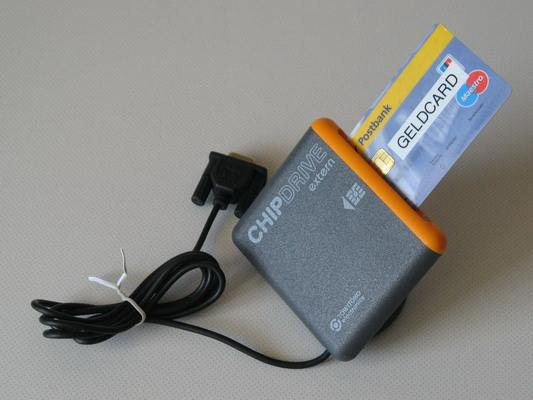
\includegraphics[width=0.95\textwidth]{images/chipdrive.jpg}
  \begin{flushright}
  \hspace*{15pt}\hbox{\scriptsize Credit:\thinspace{\small\itshape Thiemo Schuff (CC BY 3.0 DE)}}
\end{flushright}
  \captionof{figure}{Contact smart card and reader.}
  \label{fig:nfccard}
\end{figure}

\subsection{Communication standard for smart cards}
\label{sec:communicationstandard}
Application Protocol Data Unit (APDU) is a standard that describes how a smart card application should communicate with other applications (off-card) and is defined by ISO7816-4 \cite{iso7816-4}. There are two types of APDU messages: Command APDU and Response APDU \cite[~Ch. 8.3, Message Structure: APDUS]{smartcardHandbook}.

Command APDU is split into header and body. Refer to table \ref{tbl:cmdAPDU} for instruction explanation and summary. The header is mandatory for all transactions and consists of 4 bytes that is split into CLA, INS, P1 and P2. The body of a Command APDU is split into 3 parts; LC, Payload and LE. LC is 1 byte, payload is maximum 255 bytes and LE is 1 byte.

Newer smart cards supports Extended APDU which allows the payload to be up to a maximum of 65535 bytes. If the payload data is greater than 255 bytes LC must be 3 bytes where the first byte is 0x00 to denote that the APDU is extended and the remaining 2 bytes denotes the length. If extended APDU is used then LE consists of 2 bytes to account for longer responses.
\begin{table}[h!]
\caption{Command APDU layout.}
\label{tbl:cmdAPDU}
\centering

    \begin{tabular}{ | l | c | l |}
        \hline
        \thead{Name}
        & \thead{Number of bytes}
        & \thead{Description} \\ \hline

        CLA  & 1 & Command type class, type of command \\ \hline
        INS & 1 & Instruction code, command to run \\ \hline
        P1 & 1 & Free parameter \\ \hline
        P2 & 1 & Free parameter \\ \hline
        LC & 0, 1 or 3 & Length of payload \\ \hline
        Payload & 0 - 65535 & Payload data \\ \hline
        LE & 0, 1 or 2 & Expected response length \\ \hline

    \end{tabular}

\end{table}


Most Command APDUs falls into three abstract categories. The first category is retrieving something stored on the smart card. Often this command does not need any extra data (payload) and is characterized by INS, P1 and P2 deciding what data that is desired, and LE deciding what length the response is. For example: we have a smart card applet and in the instruction 01 01 00 we have stored a 8 byte variable that we want to retrieve (LE is 08). In this case the payload is empty since our theoretical method does not need any payload, but we will need to explicitly state that in the command APDU (LC is 00). The Command APDU would then look like:

\begin{table}[h!]
\centering
    \begin{tabular}{ | c | c | c | c | c | c | c |}
        \hline
        \thead{CA}
        & \thead{INS}
        & \thead{P1}
        & \thead{P2}
        & \thead{LC}
        & \thead{Payload}
        & \thead{LE} \\ \hline

        80 & 01 & 01 & 00 & 00 &  & 00 \\ \hline

    \end{tabular}

\end{table}

The second category is storing variables on the smart card. The characteristics of the Command APDU differ from the first category by having a LC and payload, but rarely needs any response apart from ``success'' or ``failure''. For example our smart card applet let's us store 8 byte in the instruction 01 02 00. LC would then be 08 and the payload would contain the 8 bytes we want to store. We set LE to 02 as we define 9000 as success and 0999 as failure. The Command APDU would then look like:

\begin{table}[h!]
\centering
    \begin{tabular}{ | c | c | c | c | c | c | c |}
        \hline
        \thead{CA}
        & \thead{INS}
        & \thead{P1}
        & \thead{P2}
        & \thead{LC}
        & \thead{Payload}
        & \thead{LE} \\ \hline

        80 & 01 & 02 & 00 & 08 & 5964574e704a593d & 02 \\ \hline

    \end{tabular}

\end{table}

The third category is sending data to the smart card and have the smart card process the data. In context of security the best example of this category is cryptographic functions. This category will use all variables of a Command APDU (INS, P1 and P2 usage depends on application complexity). As an example let us say that we want to send a Command APDU that request the ciphertext of a clear text. The instruction is 01 03 00 and our cipher algorithm in this case is very basic and ``increments'' byte values. LC and LE is 8 byte. The Command APDU would then look like:

\begin{table}[h!]
\centering
    \begin{tabular}{ | c | c | c | c | c | c | c |}
        \hline
        \thead{CA}
        & \thead{INS}
        & \thead{P1}
        & \thead{P2}
        & \thead{LC}
        & \thead{Payload}
        & \thead{LE} \\ \hline

        80 & 01 & 03 & 00 & 08 & 5964574e704a593d & 08 \\ \hline

    \end{tabular}

\end{table}

Response APDU is split into body and response trailer. The body consist of the response data and is at maximum 255 bytes or 65535 bytes depending on if extended APDU is used. All Response APDUs must contain a response trailer of two bytes which denotes the processing status (error, success, wrong format, etc.) of the Command APDU. Refer to table \ref{tbl:rspAPDU} for definitions and summary.
\begin{table}[h!]
\caption{Response APDU layout.}
\label{tbl:rspAPDU}
\centering

    \begin{tabular}{ | l | c | l |}
        \hline
        \thead{Name}
        & \thead{Number of bytes}
        & \thead{Description} \\ \hline

        Response & 0-65535 & Response data \\ \hline
        SW1+SW2 & 2 & Command processing status \\ \hline

    \end{tabular}

\end{table}


If everything is successful when processing a Command APDU with no expected response data the Response APDU may look like:

\begin{table}[h!]
\centering
    \begin{tabular}{ | c | c | c |}
        \hline
        \thead{Response data}
        & \thead{SW1}
        & \thead{SW2} \\ \hline

         & 90 & 00 \\ \hline
    \end{tabular}
\end{table}
If we use the example from the third category of Command APDUs that used ciphering as an example the Response APDU would look like:
\begin{table}[h!]
\centering
    \begin{tabular}{ | c | c | c |}
        \hline
        \thead{Response data}
        & \thead{SW1}
        & \thead{SW2} \\ \hline

        6065584f714b603e & 90 & 00 \\ \hline
    \end{tabular}
\end{table}

To better understand when to use the Command APDUs and when to use Response APDUs can use the following example: A locked door has a card reader connected to it. A person walks up to the door and presents his contactless smart card to the reader. The card reader sends a Command APDU to the card asking for the ID. The smart card processes the Command APDU and sends a Response APDU back to the card reader containing the ID of the person. This example is visualized in figure \ref{fig:doornfc} and in figure \ref{fig:doornfcapdu} we have the same example, but with actual APDU commands.

\begin{figure}[h!]
  \captionsetup{justification=centering,margin=1.5cm}
  \caption{Door lock using smart card to unlock.}
  \label{fig:doornfc}
  \centering
    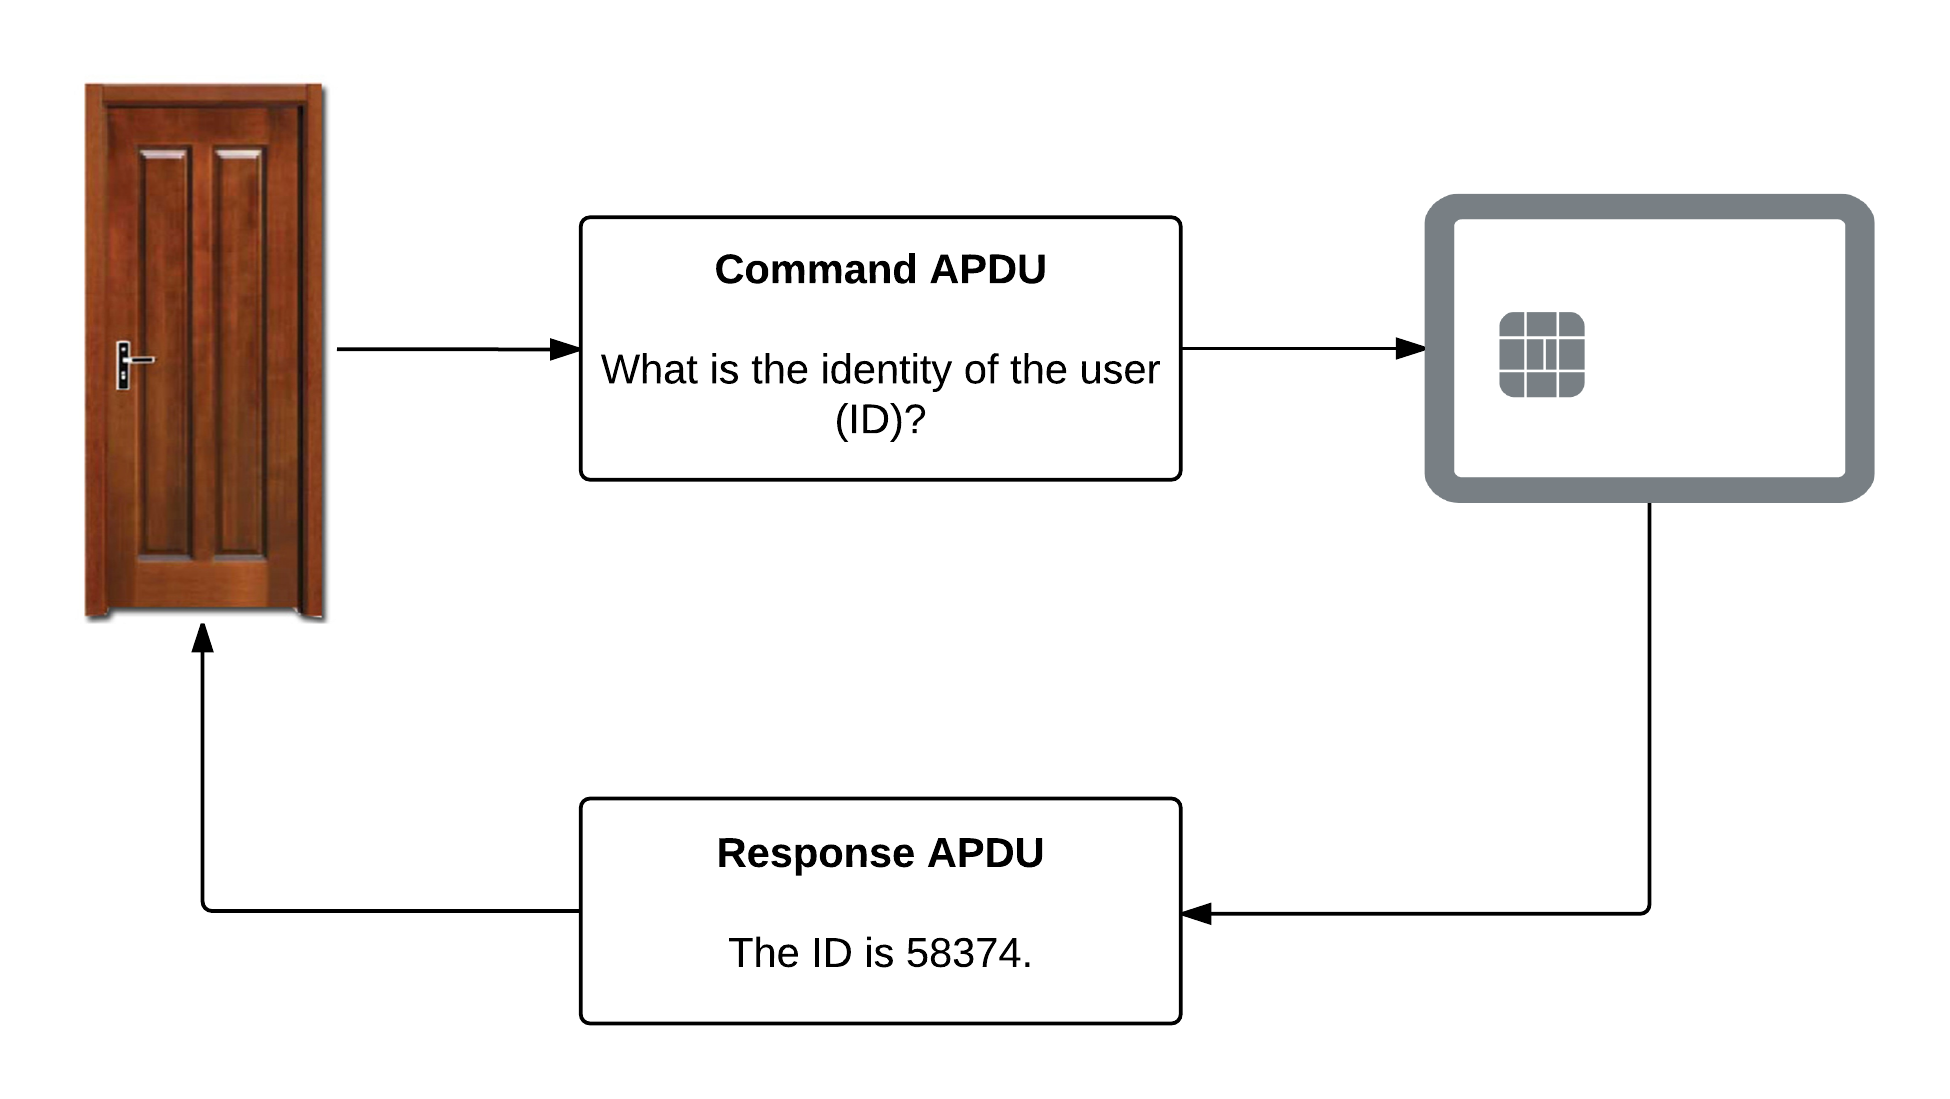
\includegraphics[width=0.95\textwidth]{images/doornfc.png}
\end{figure}


\begin{figure}[h!]
  \captionsetup{justification=centering,margin=1.5cm}
  \caption{Door lock using smart card to unlock with corresponding APDU commands}
  \label{fig:doornfcapdu}
  \centering
    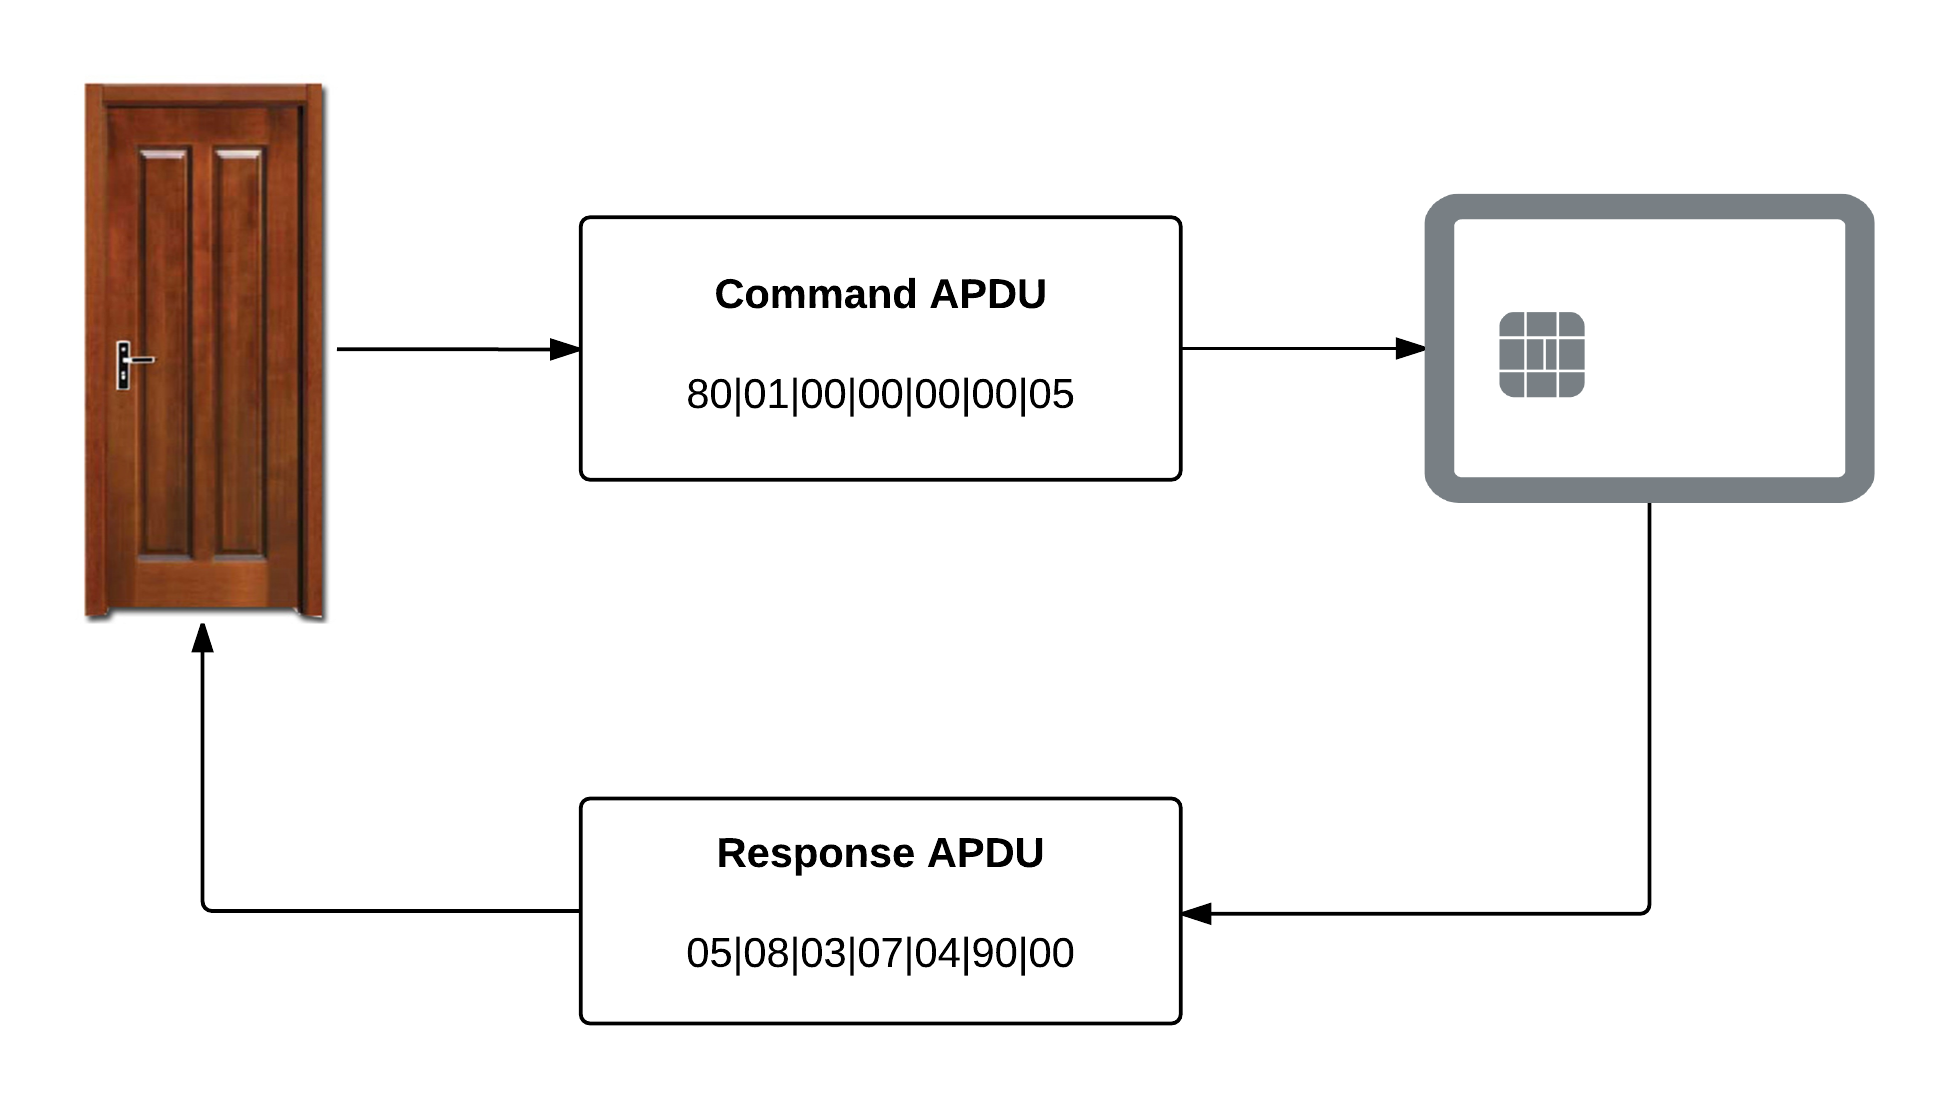
\includegraphics[width=0.95\textwidth]{images/doornfc_apdu.png}
\end{figure}

On most smart cards there is an application manager which listen for a special type of Command APDU: a Select APDU. The Select APDU contains information on what type of smart card application a sender is trying to communicate with and the job of the application manager is to activate the correct application. Before communicating with a smart card the sender should send out a Select APDU, if this step is skipped you run the risk of sending information to the wrong smart card application. A Select APDU sent to a smart card with application ID ``0102030405060708090007'' is defined as:

\begin{table}[h!]
\centering
    \begin{tabular}{ | c | c | c | c | c | c | c |}
        \hline
        \thead{CA}
        & \thead{INS}
        & \thead{P1}
        & \thead{P2}
        & \thead{LC}
        & \thead{Payload}
        & \thead{LE} \\ \hline

        00 & A4 & 04 & 00 & 0B & 0102030405060708090007 &  \\ \hline

    \end{tabular}

\end{table}

\subsection{Java Card}
\label{sec:javacard}
In section \ref{sec:smartcard} we described that smart cards are able to store data as well as process input and output. All smart cards have their own operating system that allows developers to write applications that run on the smart cards. Smart cards are not limited to one applications per card, but are able to have multiple applications installed. Traditionally it was not feasible to create programs that ran on different smart cards as the micro processors were manufacturer specific \cite{javacardapplet}. This created an environment where smart card issuers and their developers were locked to a specific manufacturer.

In figure \ref{fig:smartcardArchitecture} we can see how the architecture of a smart card is built up. In the bottom we have the hardware of the smart card which includes the ROM, EPROM, RAM and in the case of NFC cards the NFC receiver. On top of the hardware is the operating system of the smart card. The operating system has drivers installed along with API which it provides to the virtual machine. On top of the virtual machine multiple applets are able to run as mentioned above.
\begin{figure}[h!]
  \caption{Smart card architecture}
  \label{fig:smartcardArchitecture}
  \centering
    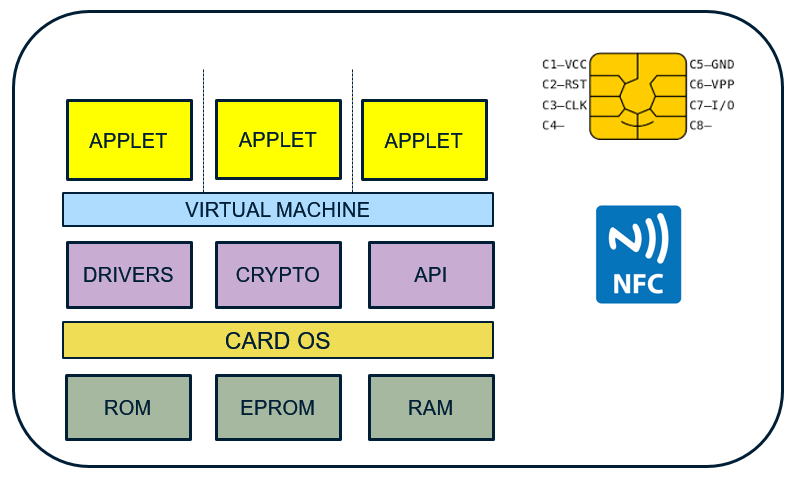
\includegraphics[width=0.95\textwidth]{images/javacardArchitecture.png}
\end{figure}

The company Schlumberger \cite{schlumberger}, later joined by Sun Microsystems \cite{sunMicroSystems}, outlined Java Card 1.0. Java Card were to alleviate the problem of manufacturer specific code and to let developers write generic applications. Newer Java Card version includes a development kit that provides a test environment and a converter tool that prepares the Java Card applet/program for installation onto a smart card. The newest Java Card version is currently 3.0.5 \cite{javacard305}.

The Java Card language is in practice a very basic version of the standard Java language. Many Java classes and features are not present. For example: int, double, long, java.lang.SecurityManager, threading and object cloning \cite{javacardlimits}. The structure of the applets differs from standard Java applets. All Java Card applets must implement:
\begin{itemize}
    \item \texttt{void install (byte [] barray, short bOffset, byte bLength)}
    \item \texttt{void process(APDU apdu)}.
\end{itemize}
\texttt{Install} is invoked when the applet is downloaded onto the smart card and should register and initialize the applet \cite{javacardinstall}. \texttt{Process} is the entry point for all requests to the application and where the applet specific logic is done \cite{javacardprocess}.

Garbage collection in the Java Card language differs from standard Java. In standard Java garbage collection is performed by the Java Virtual Machine (JVM) and runs independently of the application. In Java Card objects are stored in the persistent memory (EEPROM) and writing to this memory is very time-consuming. As a result it was decided that there would be no automatic garbage collection in Java Card and that garbage collection should be invoked by the application itself. Deciding when to perform garbage collection is very difficult as on one side it is resource intensive, while on the other side you may risk running out of memory.

%When incorporating the features of a smart card with a mobile device it would be beneficial to not rely on an external contact card or contactless card.
%One of the key features of the Java Card language is that the software is able to run on technological different smart cards. As such it is possible to deploy the Java Card applet to special micro SD memory cards. This essentially enables the smart card to be integrated with the mobile device, but at the same time be an external runtime environment. Figure \ref{fig:msdcard} is a micro SD memory card produced by Gemalto.
The fact that there is now a standardized smart card platform based on Java Card technology, means that once an applet as been written, it can be easily installed on different types of smart cards. For instance cards in micro SD format as shown in Figure \ref{fig:msdcard} and cards as shown in figure \ref{fig:nfccard} would be able to run the same application (given that both support Java Card).


\begin{figure}[h!]
  \caption{Micro SD card from Gemalto.}
  \label{fig:msdcard}
  \centering
    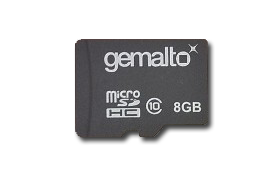
\includegraphics[width=0.75\textwidth]{images/msd.png}
\end{figure}


\subsection{Other smart card programming languages}
Besides Java Card, another widespread smart card operative system is MULTOS \cite{multos}. MULTOS was the first open high security operating system that supported multiple applets and supports the programming languages native assembly (MEL), C and Java. Java Card and MULTOS differs from how they handle applets shared space/memory on the smart cards. MULTOS security targets are: Applets can only be loaded by the card issuer, applets are segregated and secure package deployment. Java Card uses a secure channel to distribute applications whereas MULTOS uses secure packaging. The essence is that third parties can deploy new applets to the smart card containing sensitive data. This is possible as the package is encrypted with the public key of MULTOS (card unique) and thus you do not need a secure channel \cite{smartcardThesis, multosVSjavacard}.

There exists a .NET version of a smart card OS started by Microsoft which led to other versions developed by Gemalto and CardWerk. We will use Java Card in this thesis as this is supported by our smart cards and is similar to standard Java which is used in our mobile devices (refer to section \ref{sec:androidOS}).

\section{Android operating system}
\label{sec:androidOS}
Mobile operating system refers to the operating system running on a mobile device (smartphones, GPS devices, tablets, etc.). In this thesis we will focus mainly on smartphones and tablets since their capabilities are within our scope and the fact that they often share the same operating system.

Android is an open source licensed mobile operating system and is based on one of the LTS (long-term support) branches of the Linux kernel. Google Inc. \cite{google} is the current developer of the mobile operating system and their primary focus has been smartphones and tablets. In later years Google has put resources into incorporating Android with TVs, wrist watches and cars. In 2015 Q2 82,8 \% of smartphones worldwide was shipped with a version of the Android mobile operating system \cite{androidMarketShare}.

The Android mobile operating system supports applications that are written in Java, GO and C/C++. The applications run in their own sandbox with their own allocated memory space, but applications can also access shared resources given permission to do so by the user.

For practical reasons and because of time constraints we have restricted us to one mobile operating system. The mobile operating system of choice is Android. The reason for picking Android as our mobile platform is the flexibility of the Android system and devices when it comes to secure element support. iOS devices have no support for micro SD smart cards and Windows Phones does not seem to have any libraries support smart card communication. Blackberry is an alternative, especially their latest iterations which is a custom Android version, but due to their low market share they are not representative in a ``bring your own device'' situation. We discuss the Blackberry Priv more in depth in section \ref{sec:blackberry}.

% devices as iPhone OS does not support micro SD cards and Windows Phone devices does not seem to support secure elements at all.

\subsection{Smart card support in Android}
\label{sec:supportAndroid}
In Android version 2.3 (API level 9) NFC support was added which enabled a mobile device to read NFC Data Exchange Format (NDEF) from NFC devices/tags. In Android 2.3.3 (API level 10) the class \texttt{IsoDep} was added which enabled mobile devices to send byte data via NFC to devices with NFC support. This means that any device supporting API level 10 or higher and with a NFC adapter can communicate with smart cards via NFC.

As mentioned in section \ref{sec:javacard} smart card applications can run on micro SD cards. Mobile devices with a micro SD card slot can in theory communicate with these types of smart cards, but Android has no native support for communicating with them. This essentially means that the hardware is there on some mobile devices, but developers lack the bridge between their application to the hardware.

The Secure Element Evaluation Kit (SEEK) for the Android platform is an open source project, maintained by Giesecke \& Devrient GmbH \cite{Giesecke}, which have a vision to make it easier to use secure elements in Android applications. The framework enables access to a variety of secure elements such as SIM cards, micro SD cards and embedded secure elements. Their final goal is to have their library as an integrated part of the Android operating system such that all new mobile devices comes with hardware-backed security support \cite{SEEK}. Some mobile device manufactures have included this framework, but there exists no documentation stating which devices have it, what channels are open and how to access the secure elements. Often the case is that only the channel to the mobile device SIM card is open meaning you cannot access custom secure elements.

Since SEEK for Android is open source and we can look into how the software works (although this require resources), but if the pre-installed operating system does not have it installed we will need to build our own version and flash the device. Running a custom version of an operating system requires the organization to maintain and support it. From a security standpoint this is not viable as you will not automatically get security updates and will be running an unofficial version of an operating system. Running a custom operating system may also cause issues for the users as some services may block the user if they detect it (banking applications, proprietary applications, etc.).

As an alternative to flashing the operating system one can use proprietary drivers from smart card manufacturers. Gemalto produces a Java library, IDGo800, which is a cryptographic and communication middleware for their smart cards (more on this in section \ref{sec:gemaltoApp}). Installing/using third-party applications/libraries to communicate with smart cards may not always be the best option, as you make yourself dependent on a third-party. In essence, opting for this solution results in a vendor lock. Security wise you should not blindly trust a third-party and you may not have access to the software if you wish to evaluate it.

\subsection{Blackberry Priv}
\label{sec:blackberry}
The Blackberry Priv by Blackberry is branded as a ``secure smartphone'' \cite{blackberryPriv}. Blackberry's states that all data on the device is hardware-encrypted, the operating system performs a integrity check every time it boots, and that Blackberry's hardware suppliers are to be trusted. Blackberry Priv runs a modified Android version and comes with native secure element support. What this entails is that the Blackberry Priv may be the ``off-the-shelf'' solution we seek for both hardware and software (operating system) as we do not need to run and maintain custom frameworks or flash the operating system to communicate with secure elements as discussed in section \ref{sec:supportAndroid}.

The downside of opting for the Blackberry Priv is that we lock ourselves to a specific vendor which defeats the ``bring your own device'' concept. Another thing to keep in mind is that this is one single device, meaning it would need to be reviewed as to whether it fits the organization needs in terms of functionality and other characteristics (size, weight, battery, etc.). The device is also rather expensive compared to devices with similar specifications.

In this thesis we will not seek further investigation on the Blackberry Priv and we will focus on more standardized smartphones, but it is important to know that it exists for future research. Information on our test device can be found in the chapter \ref{ch:testing}, section \ref{sec:equipment}.

%The Secure Element Evaluation Kit (SEEK) for the Android platform is an open source project, maintained by Giesecke \& Devrient GmbH \cite{Giesecke}, which have a vision to make it easier to use secure elements in Android applications. The framework provides access to a variety of secure elements such as SIM cards, micro SD cards and embedded secure elements. Their final goal is to have their library as an integrated part of the Android operating system such that all new mobile devices comes with hardware-backed security support \cite{SEEK}.

%Since SEEK for Android is open source and we can look into how the software works (although this require resources), but if the pre-installed operating system does not have it installed we will need to build our own version and flash the device. Running a custom version of an operating system requires the organization to maintain and support it. From a security standpoint this is not viable as you will not automatically get security updates and will be running an unofficial version of an operating system. Running a custom operating system may also cause issues for the users as some services may block the user if they detect it (banking applications, proprietary applications, etc.).

\section{Cryptography}
%What is cryptography?
Cryptography is a method for protecting confidential data using complex mathematics and computer science. Most cryptographic functions/algorithms relies heavily on the fact that the mathematics are so complex that they are ``unbreakable'' without knowledge of the encryption/decryption key.

\subsection{Public-key cryptography}
\label{sec:publicKeyCrypto}
Public-key cryptography refers to a set of methods for asymmetric cryptography. It is based on the concept that one entity (user, server, etc.) generates a key pair consisting of one public key and one private key. Data encrypted using the public key can only be decrypted by the private key and due to the complexity of the keys it is improbable that the private key can be generated from the public key. The public key, as the name suggests, is publicly available for other entities. This combination allows entities to communicate securely given that they have each others public key and their private key is stored securely. Figure \ref{fig:encrypt_basic} shows how a sender can send a message that only the receiver can read. Although it is important to note that this operation is more resource intensive and time consuming compared to symmetric key encryption/decryption.

\begin{figure}[h!]
  \captionsetup{justification=centering,margin=1.5cm}
  \caption{Asymmetric key encryption/decryption using public-private key pair.}
  \label{fig:encrypt_basic}
  \centering
    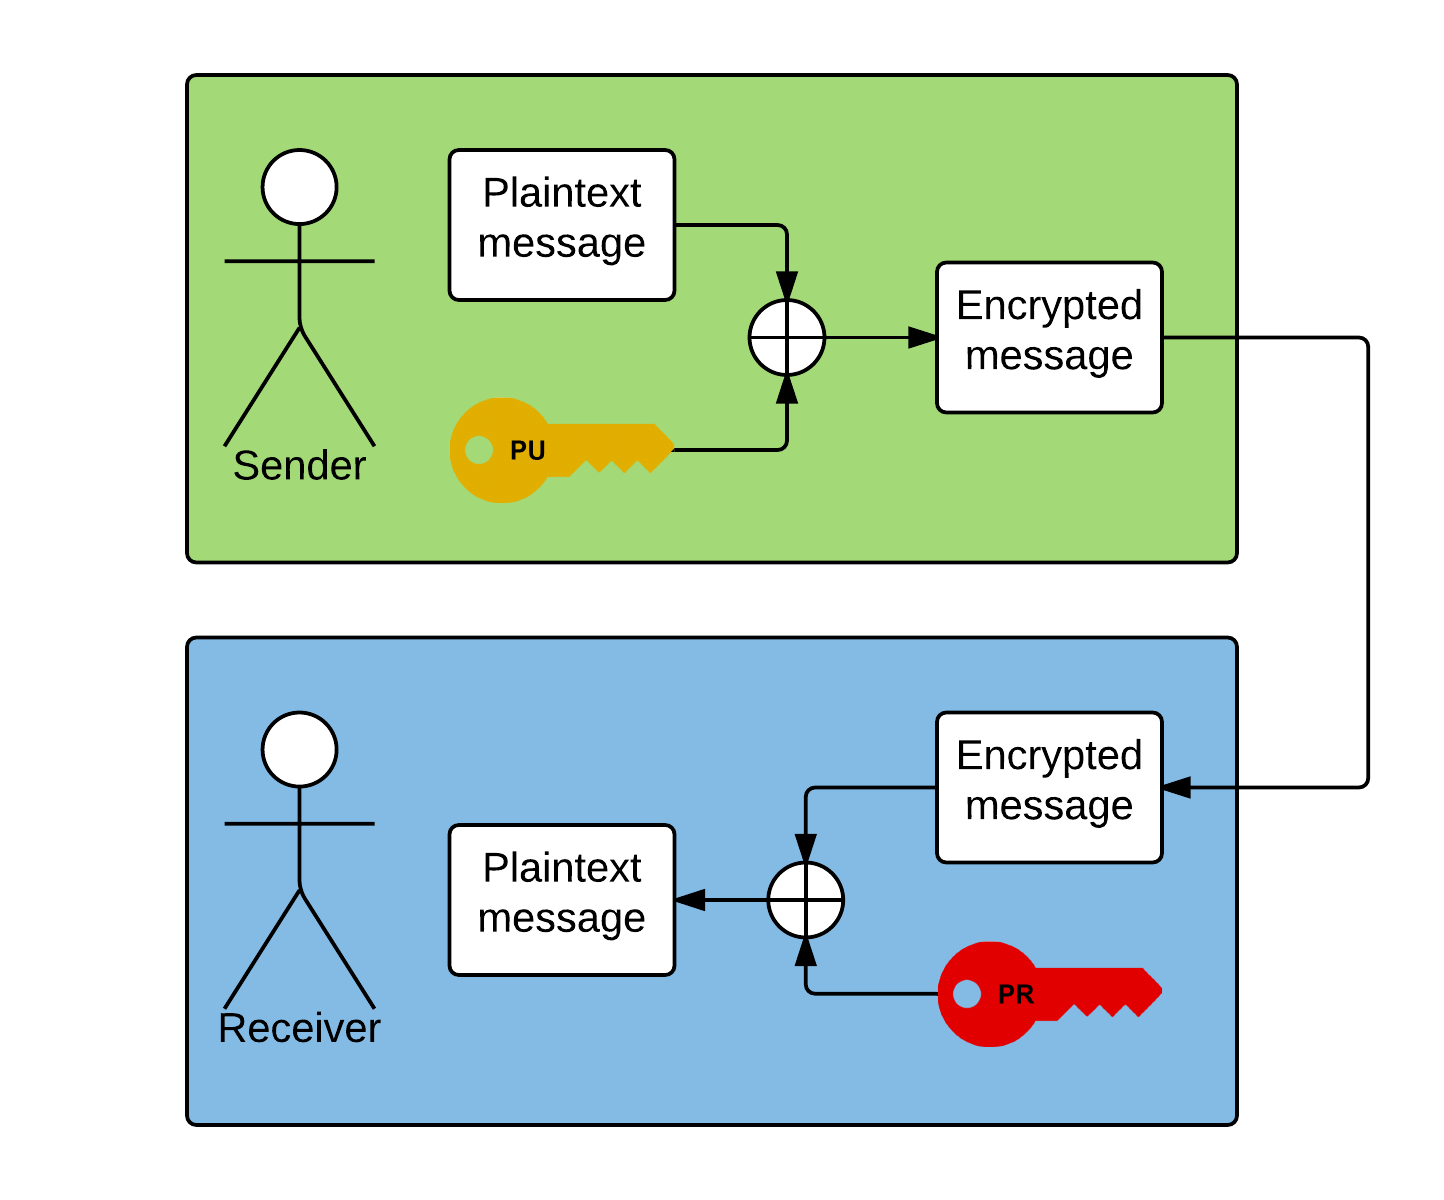
\includegraphics[width=1\textwidth]{images/encrypt_basic.png}
\end{figure}

One of the most common public-key cryptosystems is RSA, which is widely used for secure communication. RSA builds on the principle of factorization of the product of two prime numbers, or rather the difficulty of factorize the product. It is not impossible to factorize the product of two prime numbers and there was a challenge by the RSA Laboratories where one could win prizes for factorized RSA-keys \cite{rsaChallenge}, but the most complex RSA that were cracked was 768-bit. Proving that RSA is secure is out of the time scope for this thesis. Other sources conclude that with long enough keys and correct protocol implementation, the math behind RSA can be considered secure \cite[~p. 194]{cryptoMath}. Information on the inner workings of RSA can be found in the book ``Understanding Cryptography'' by Christof Paar and Jan Pelzl, chapter 7 ``The RSA Cryptosystem'' \cite{cryptoMath}.

Message authentication can also be done by public-key cryptography. First the message is hashed using a secure hash function, for instance SHA-2 \cite{shaRFC}, which creates a digest. The digest is then encrypted with the private key and the ``digital signature'' is then sent with the original message. The receiver can then verify the integrity of the message by computing the hash of the message using the same secure hash function and decrypt the ``digital signature'' using the senders public key. If they are a match the receiver can with certainty conclude that the message has not been tampered with and originates from the sender.

\begin{figure}[h!]
  \captionsetup{justification=centering,margin=1.5cm}
  \caption{Digital signing using public-private key pair.}
  \label{fig:signing_basic}
  \centering
    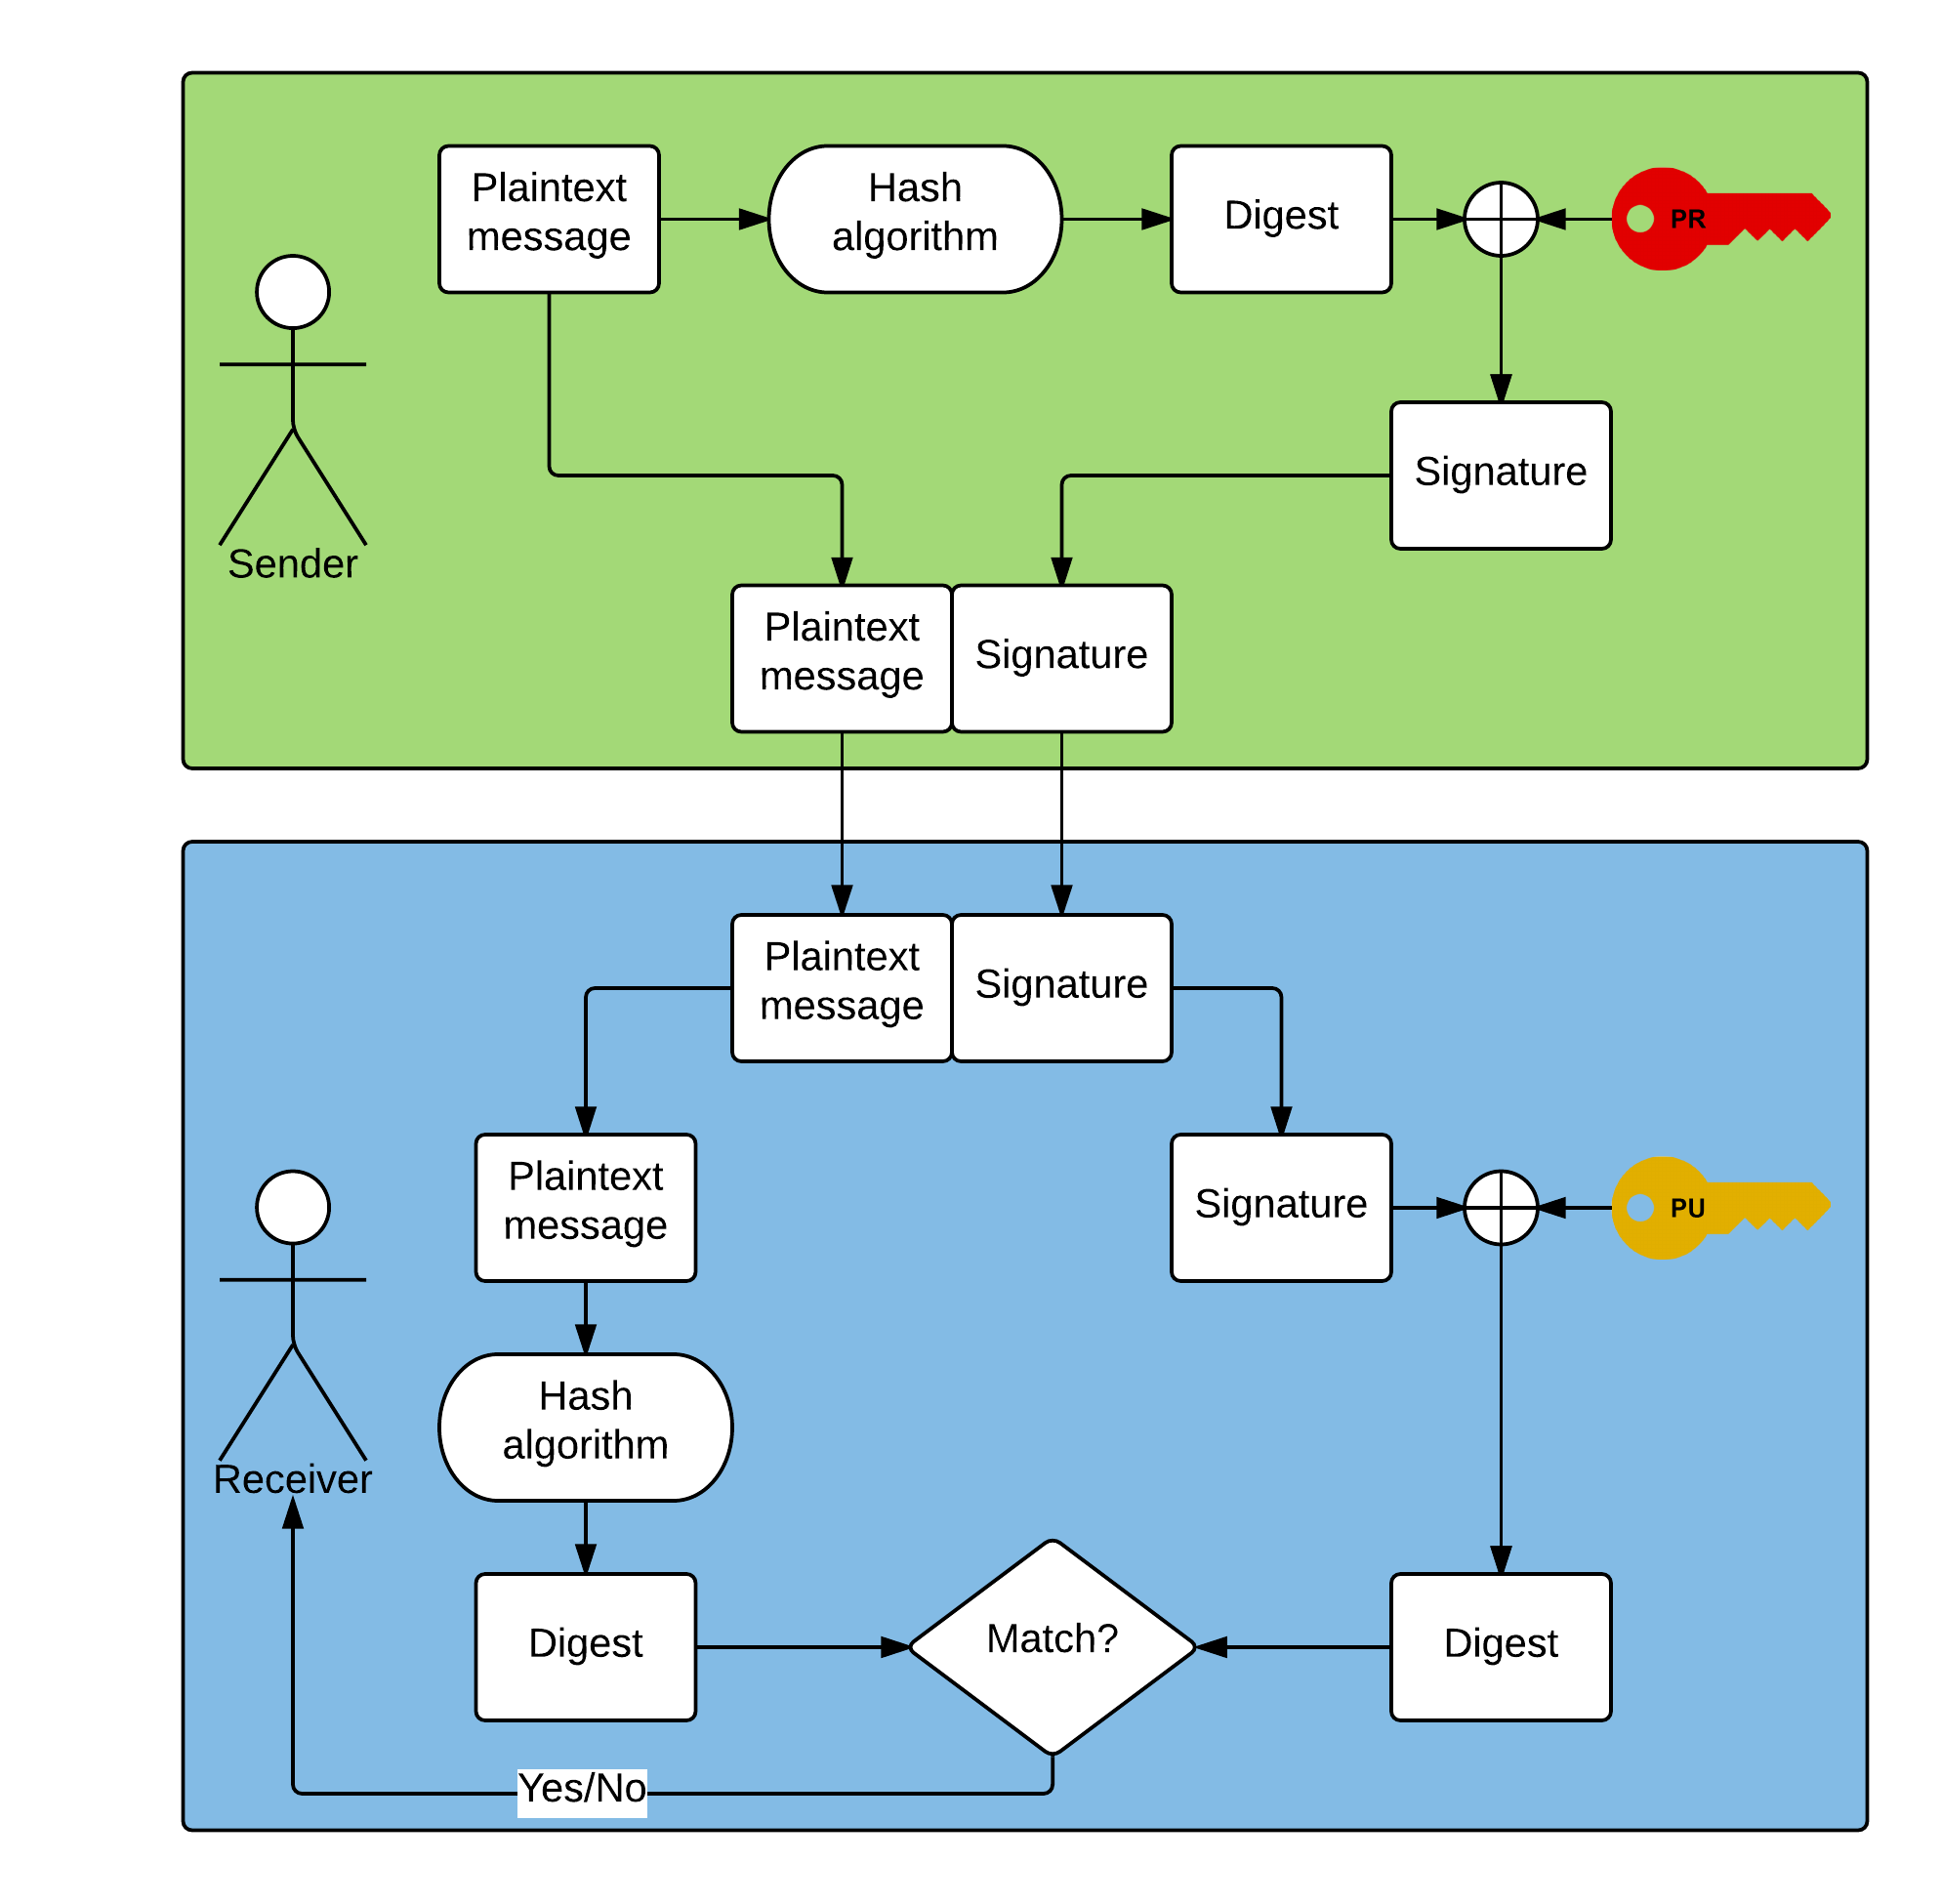
\includegraphics[width=1\textwidth]{images/signing_basic.png}
\end{figure}

One of the key issues with public-key cryptography is verifying the identity of the public key owner. Authentication is not a trivial matter and is solved by using certificates to prove that the holder of the key is who they claim to be. The certificates needs to be signed by a trusted third party whom both the sender and receiver of the message trust. The mutual trust relationship is a complex matter and is not a topic we will investigate further in this thesis, but we will assume that it is possible to achieve.

\subsection{Symmetric-key cryptography}
\label{sec:symmetricCrypto}
Symmetric-key cryptography uses the same cryptographic key for both encryption and decryption. There are two main areas of application for symmetric-key cryptography; secure storage of data and secure communication. Secure storage of data is the most straight forward of the two. An entity (user, server, etc.) generates a key, encrypts the data using the key, stores the key for future use and decrypts the data using the key whenever the entity require the data. As long as the key is stored securely and the encryption algorithm is secure the data can be stored in an unsecured environment. Secure communication using symmetric-key is similar, but instead of the same entity decrypting the data, the encrypted data is transmitted to a new entity which decrypts it using the same key. This requires the key (known in this case as shared secret) or key generation process to be known by both parties. There are two methods for symmetric-key encryption/decryption. Stream ciphering takes one byte at the time and encrypts/decrypts it whereas block ciphering takes bigger chunks of data and encrypts/decrypts the data. Both methods have their own weaknesses and strengths \cite[~Ch. 2.1.1]{cryptoMath}.

Stream ciphering is fast and relatively simplistic to implement. This along with the fact that it can encrypt byte by byte makes it very suitable for use when plaintext data comes in  unknown length and over time (streams). Areas of application includes voice chat, video feed and http communication. Disadvantages of stream ciphering is that if the algorithm is cracked then it is susceptible to insertions and modifications as well as the fact that a single plaintext symbol is represented as a single ciphertext symbol (limited alteration).

Block cipher is a more complex and requires more overhead. First of all, data must be divided into equal size blocks. The blocks cannot be too small as they would be prone to dictionary attacks and not too big as this would make the encryption/decryption process too resource intensive. In block ciphers the block size must be fixed through the encryption process. This will often result in redundant data. For example, 200-bit plaintext with a 64-bit block size will result in three blocks of 64-bit and a fourth block with only 8 bit of ``real'' data and 56 bit of redundant bits. Since block ciphering uses the previous block to cipher the current block it is possible to detect tampering and faults, but this also results that data may be lost if a block becomes corrupt.

Advanced Encryption Standard (AES) is one of the most common symmetric-key cryptography methods. AES does not rely on number factorization (opposed to RSA), but rather substitution and permutation using a key. It can be seen as hashing data and being able to reverse the hashing using the same key. There are currently no known analytic attacks against AES which are less complex than brute-force attacks and consensus is that it is secure as long as long enough keys are used.

\section{Mobile technology vulnerabilities}
Mobile technology vulnerabilities and attack vectors are numerous and before looking into how smart cards can help mitigate an alleviate threats we will need to identify and characterize them.

\subsection{Physical access}
An attacker may gain physical access to the users mobile device through theft or simply that the user misplaced the mobile device. With physical access to the device an attacker would be able to retrieve data from the device. A common defense against this is encrypting the data on the device, but this requires the keys to be stored somewhere securely. If the keys are not stored securely the result is that the data on the device may fall into the wrong hands.

Apart from encrypting the device a more basic form of protection against physical access is using screen locks along with disabling USB debugging etc. What is important to remember is that if an attacker or organization has enough time and resources they may at some point become successful in breaking these security measures. This was recently proven correct by the Federal Bureau of Investigation when they were able to hack into the iPhone 5C used by one of the ``San Bernardino shooters'' after Apple refused to help bypass the security measures \cite{iphoneHack}.

\subsection{Remote access}
An often overlooked attack vector is badly implemented applications on the mobile device. Inherently a lot of functionality is secure, but due to negligence or bad planning functionality is implemented in a bad way. This can include memory leaks, weak cryptography, open for code injections or openly exposing private data to third parties. We classify these vulnerabilities as ``remote'' vulnerabilities as an attacker rarely needs physical access to exploit them. In the ``Top 10 Mobile Risks 2014'' from OWASP \cite{OWASPTopTenMobile} most of the bullets fall under this category. For instance, client side injection allows attackers to remotely execute code on a user device by abusing poor validation of resources.

In rare cases an application with flaws may expose other applications for attacks, but there exists countermeasures to this, for instance that all applications run in their own sandbox. In Android, all applications run in their own environment and applications can only access their own resources and shared resources. The vulnerabilities mentioned above can potentially enable sharing resources that was meant to be private.

\subsection{External vulnerabilities}
External vulnerabilities differs from remote access by that external vulnerabilities are not tied to the device, they focuses on data or information in transit.

Communication is a vital part of modern systems; data is sent between devices and between devices and servers. Sensitive data requires a secure communication channel which cannot be tapped into by a third party. Secure communication on public networks involves agreeing upon encryption keys which the data should be encrypted with before being sent. Encrypting the communication channel will protect against man-in-the-middle attacks, but this requires both parties to authenticate themselves as encrypting the data won't help if you are sending the data directly to the attacker.

As mentioned above, a secure communication channel is useless if you are sending the data directly to the attacker. A vital part of communication security is being able to authenticate the parties in a communication transaction. If the attacker is able to impersonate another party by installing fake certificates on the mobile device or by tricking the user into communicating with the attacker the consequences can be of great significance. All external parties should be treated as hostile or untrusted parties until proven otherwise.

\subsection{The result of infected or compromised devices}
The type of virus or malware on an infected device can vary, some are harmless and serve more as an annoyance or trying to trick the user into visiting bogus websites, but some are more malicious and will access private files and information. From a security stand-point it is a disaster if a virus or malware is able to read and modify data which is otherwise confidential.

Often the user will not know that their mobile device is infected and some viruses or malware are very hard to detect by anti-virus. The ``2015 Cheetah Mobile Security Report'' \cite{cheetahSec} reports that the number of viruses on Android devices exceeds over 9,5 million and that the problem is growing. That there exists over 9,5 million viruses for Android shows that Android is a sought after platform to compromise.

When designing and developing applications one should take into consideration that the mobile device may be infected or compromised as well as the possibility for the device to at some point become infected or compromised.


\iffalse %COMMENT


\subsection{Infected device}
The most obvious threat to mobile devices is when the mobile device itself is infected with virus or malware. The type of virus or malware can vary, some are harmless and serve more as an annoyance or trying to trick the user into visiting bogus websites, but some are more malicious and will access private files and information. From a security stand-point it is a disaster if a virus or malware is able to read and modify data which is otherwise confidential.

Often the user will not know that their mobile device is infected and some viruses or malware are very hard to detect by anti-virus. The ``2015 Cheetah Mobile Security Report'' \cite{cheetahSec} reports that the number of viruses on Android devices exceeds over 9,5 million and that the problem is growing. That there exists over 9,5 million viruses for Android shows that Android is a sought after platform to compromise. When designing and developing applications one should take into consideration that the mobile device may be infected or compromised.

\subsection{Lost or stolen device}
An attacker may gain physical access to the users mobile device through theft or simply that the user misplaced the mobile device. With physical access to the device an attacker would be able to retrieve data from the device. A common defense against this is encrypting the data on the device, but this requires the keys to be stored somewhere securely. If the keys are not stored securely the result is that the data on the device may fall into the wrong hands.

\subsection{Insecure communication channel}
\label{sec:unsecureCommunication}
Communication is a vital part of modern systems; data is sent between devices and between devices and servers. Sensitive data requires a secure communication channel which cannot be tapped into by a third party. Secure communication on public networks involves agreeing upon encryption keys which the data should be encrypted with before being sent. Encrypting the communication channel will protect against man-in-the-middle attacks, but this requires both parties to authenticate themselves as encrypting the data won't help if you are sending the data directly to the attacker. More on this in section \ref{sec:authenticationChallenges}.

\subsection{Authentication challenges}
\label{sec:authenticationChallenges}
%Are people who they say the are?
As mentioned in section \ref{sec:unsecureCommunication} a secure communication channel is useless if you are sending the data directly to the attacker. A vital part of communication security is being able to authenticate the parties in a communication transaction. If the attacker is able to impersonate another party by installing fake certificates on the mobile device or by tricking the user into communicating with the attacker the consequences can be of significance.

\subsection{Insecure applications}
An often overlooked attack vector is badly implemented applications on the mobile device. Inherently a lot of functionality is secure, but due to negligence or bad planning are implemented in a bad way. This can include memory leaks, weak cryptography, open for code injections or openly exposing private data to third parties. In rare cases an application with flaws may expose other applications for attacks, but there exists countermeasures to this, for instance that all applications run in their own sandbox. In the ``Top 10 Mobile Risks 2014'' from OWASP \cite{OWASPTopTenMobile} most of the bullets fall under this category.
\fi %UNCOMMENT
